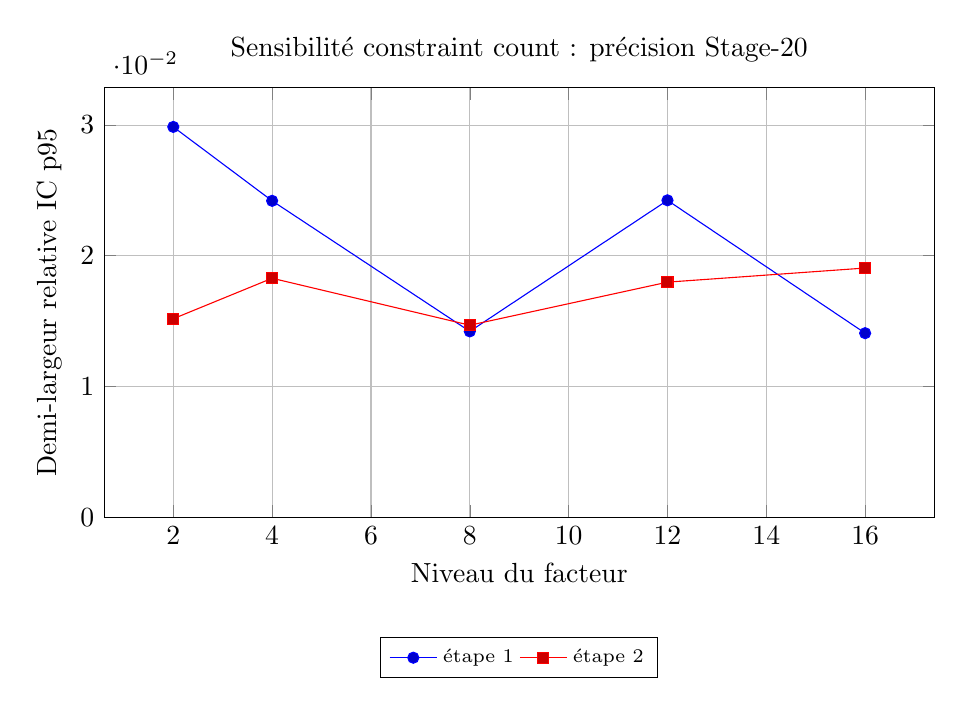
\begin{tikzpicture}
\begin{axis}[width=\linewidth,
height=0.58\linewidth,
title={Sensibilité constraint count : précision Stage-20},
xlabel={Niveau du facteur},
ylabel={Demi-largeur relative IC p95},
grid=major,
legend style={font=\scriptsize,at={(0.5,-0.28)},anchor=north,legend columns=2},
ymin=0]
\addplot+[mark=*] coordinates {(2.0,0.02986000137861953) (4.0,0.02420195483336553) (8.0,0.014211446509459035) (12.0,0.02424101696366615) (16.0,0.014073779021601897)};
\addlegendentry{étape 1}
\addplot+[mark=square*] coordinates {(2.0,0.015179910923108341) (4.0,0.018277528664099717) (8.0,0.014683287087945808) (12.0,0.017979856939250968) (16.0,0.01905925110471172)};
\addlegendentry{étape 2}
\end{axis}
\end{tikzpicture}
